Una caratteristica davvero interessante di Docker è il modo in cui viene gestito il file system. Docker utilizza un’implementazione di \href{https://en.wikipedia.org/wiki/UnionFS}{\textbf{Union File System}} per comporre il file system che apparirà visibile al container. Gli Union File System (ad esempio UnionFS o \href{https://en.wikipedia.org/wiki/Aufs}{\textbf{aufs}}) consentono di unire diversi file system e montarli in un unico punto di mount.\\
Un'immagine Docker è in realtà un insieme di file organizzati in directory: in definitiva, è un file system. Un'immagine docker può essere costruita sulla base di un'immagine già esistente semplicemente aggiungendo e/o modificando alcuni file ad esempio facendo commit di un immagine gia esestende oppure agguingendo strati con il dockerfile. E questo può essere ripetuto per un numero illimitato di volte. Un'immagine può essere ad esempio costituita da $n$ strati (vedi figura: \ref{img:container}): questo concetto è conosciuto anche come “immagini stratificate” \href{http://goo.gl/z1ne3Q}{(\textbf{layered})}. Nell’esempio precedente, quando l’immagine Docker va in esecuzione, i $n$ file system vengono uniti insieme (merge) in modalità sola lettura, e ad essi viene sovrapposto un ulteriore strato in modalità lettura–scrittura writable layer (vedi fig: \ref{img:container}).
\begin{figure}[H]
	\begin{center}
		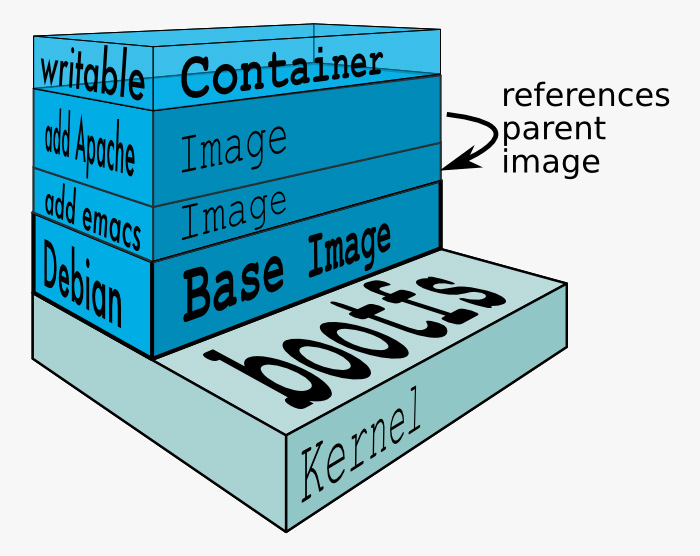
\includegraphics[width=0.99\columnwidth]{img/ContainersOperations-2_fig02.jpg}
		\caption{Un file system stratificato (layered file system).}
		\label{img:layered}
	\end{center}
\end{figure}
Se due container condividono parte degli strati dell’immagine, questi layer non dovranno essere replicati nel file system host, poiché sono montati in modalità sola lettura. Questo può generare significativi risparmi specie se un’azienda si dà una certa disclipina riguardo al modo in cui possono essere create le immagini: potrebbe essere il caso, ad esempio, di stabilire che tutte le immagini debbano derivare da una base comune.\\In questo caso, siccome la base comune sarà probabilmente lo strato che prende la maggior parte dello spazio disco e gli altri layer dovranno aggiungere installazioni o configurazioni minori, tale semplice linea guida potrebbe far risparmiare grandi quantità di spazio disco. Come in figura (\ref{img:layered}) l'immagine di base condivisa fra vari container potrebbe essere quella del layer che comtiene l'immagine Debian. 
